\section{Nota teórica}
En esta sección se describen los componentes principales que se utilizaron para el desarrollo de un sismógrafo.
\subsection*{STM32F429 Discovery kit}
Este microcontrolador permite a los usuarios desarrollar fácilmente aplicaciones de alto desempeño. Incluye un ST-LINK/V2 embebido como una herramienta de depuración, una SRAM externa de 64-Mbit, un ST MEMS giroscopio, un USB OTG conector AB, LEDs y botones. Algunas de las características generales se resumen a continuación.

\subsubsection*{Características generales}
Las características más importantes de este mcu se mencionan a continuación:
\begin{multicols}{2}
 \begin{itemize}
    \item 2.4 QVGA TFT LCD.
    \item 64-Mbit SDRAM.
    \item USB OTG con conector Micro-AB.
    \item Header para LQFP144 I/Os.
    \item Sensor de movimiento I3G4250D, Giroscopio ST MEMS de 3-ejes-
    \item On-board ST-LINK/V2-B.
    \item Alimentación por USB o fuente externa de \SI{3}{\volt} o \SI{5}{\volt}.
    \item 2  push-button (Usuario y reset).
    \item Core: ARM 32 bits Cortex-M4 con FPU (RISC).
    \item Debug: SWD, JTAG.
    \item Trabaja en frecuencia de \SI{180}{\mega\Hz}
    \item 168 I/O con capacidad de interrupción.
    \item 2MB flash, 256 KB SRAM.
    \item Controlador LCD-TFT.
    \item 21 interfaces de comunicaciones(I2C,USART,SPI,SAI,CAN).
    \item Low Power.
    \item Conectividad avanzada USB 2.0.
    \item Intefaz de camara.
    \item 2x12bit convertidor D/A.
    \item True RNG.
    \item CRC.
    \item 6 LEDS: LD1 (USB Comms), LD2(3.3V PowerOn, 2 LEDS de ususario (LD3 y LD4), 2 LEDS USB OTG (LD5 y LD6).
    \item Controladores DMA.
    \item 17 timers: 12 timers de 16bit, 2 de 32bit de hasta 180MHz, c/u con 4IC/OC/PWM.
\end{itemize}   
\end{multicols}

\subsubsection*{Diagrama de bloques}
En la figura \ref{fig1} se muestra el diagrama de bloques del STM32F429.
\begin{figure}[H]
\centering
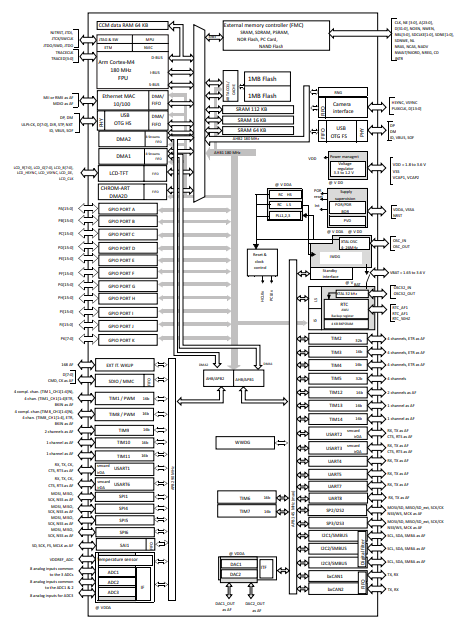
\includegraphics[width=.55\linewidth]{Imagenes/1.png}
 \caption{Diagrama de bloques del STM32F429 . Tomado de \cite{web}.}
 \label{fig1}
\end{figure}
\subsubsection*{Diagrama de pines}
Luego, el diagrama de pines de este mcu se presenta en la figura \ref{fig2}
\begin{figure}[H]
\centering
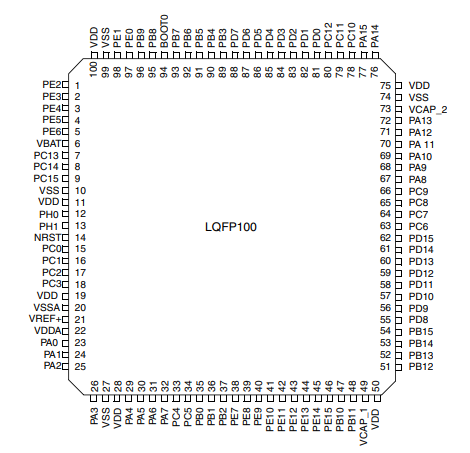
\includegraphics[width=.55\linewidth]{Imagenes/2.png}
 \caption{Diagrama de pines del STM32F429. Tomado de \cite{web}.}
 \label{fig2}
\end{figure}
\subsubsection*{Características eléctricas}
Las siguientes tablas resumen las características eléctricas de este microcontrolador.
\begin{figure}[H]
\centering
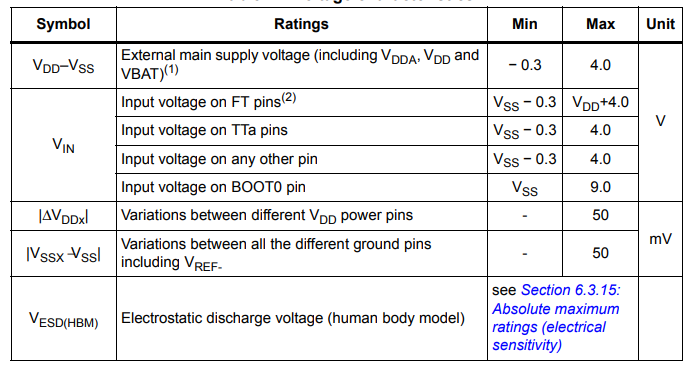
\includegraphics[width=.55\linewidth]{Imagenes/3.png}
 \caption{Detalles del voltaje del mcu. Tomado de \cite{web}.}
 \label{fig3}
\end{figure}

\begin{figure}[H]
\centering
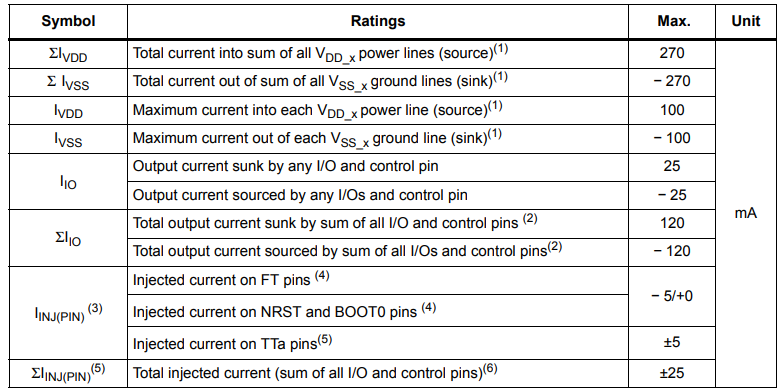
\includegraphics[width=.55\linewidth]{Imagenes/4.png}
 \caption{Detalles de la corriente en el mcu. Tomado de \cite{web}.}
 \label{fig4}
\end{figure}


\subsection*{Periféricos utilizados}
Los registros utilizados en este laboratorio se describen a continuación:
\begin{itemize}
    \item WHO\_AM\_I: Registro utilizado como identificador.
    \item CTRL\_REG1: Registro utilizado para habilitar registros de lectura de ejes.
    \begin{figure}[H]
        \centering
        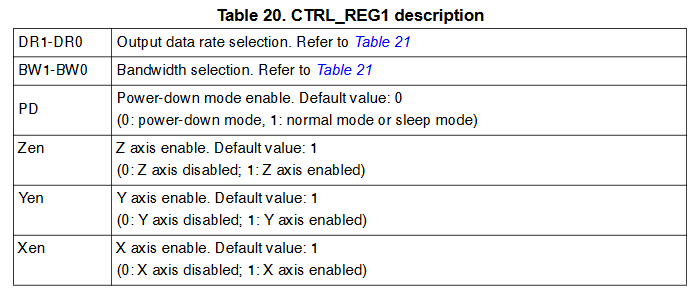
\includegraphics[width=.7\linewidth]{Imagenes/k1.png}
        \caption{Descripción del registro CTRL\_REG1. Tomado de \cite{l3gd20}.}
        \label{fig5}
    \end{figure}
    \item CTRL\_REG4: Este registro es utilizado para la configuración del DPS y también para la configuración del modo de selección del SPI.
    \begin{figure}[H]
        \centering
        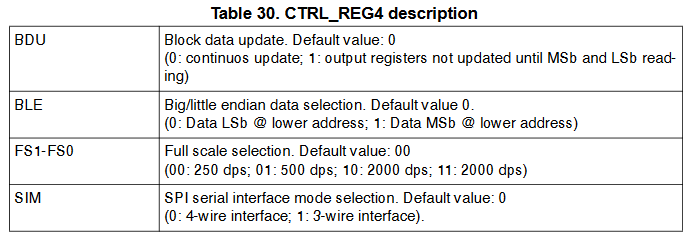
\includegraphics[width=.7\linewidth]{Imagenes/k2.png}
        \caption{Descripción del registro CTRL\_REG4. Tomado de \cite{l3gd20}.}
        \label{fig6}
    \end{figure}
    Para la lectura de los ejes, se utilizan los siguientes registros, ambos son registros de 8 bits. La \textbf{L} es para representar los primeros 8 bits menos significativos y la \textbf{H} para los 8 bits más significativos, ambos de la lectura del giroscopio en el eje indicado (X, Y o Z).
    \item OUT\_X\_L y OUT\_X\_H
    \item OUT\_Y\_L y OUT\_Y\_H
    \item OUT\_Z\_L y OUT\_Z\_H
    \item STATUS\_REG
    \begin{figure}[H]
        \centering
        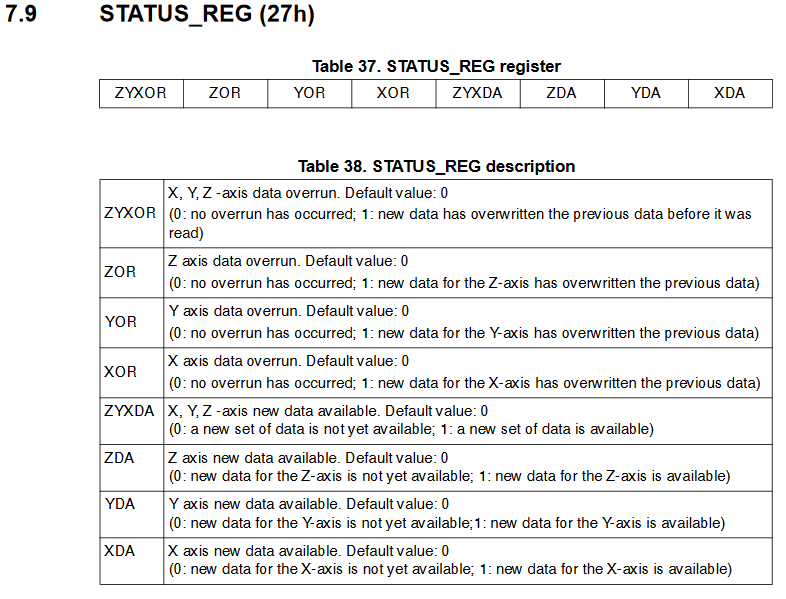
\includegraphics[width=.7\linewidth]{Imagenes/k3.png}
        \caption{Descripción del registro STATUS\_REG. Tomado de \cite{l3gd20}.}
        \label{fig7}
    \end{figure}
\end{itemize}

\subsection*{Componentes electrónicos complementarios}
% quiza mencionar la ayuda de la protoboard, en realidad fue como lo único.
Es un circuito que lo compone una electrónica básica (así lo resume la tabla \ref{table_2}), solo se usó una protoboard y 3 resistencias en total, una batería de \SI{9}{\volt}, esto para realizar un divisor de tensión con el objetivo de alimentar a la placa STM32249 Discovery Kit con \SI{5}{\volt}. Así, se sabe que $v_{out} \approx \SI{5}{\volt}$
\begin{itemize}
\item $R_1 = \SI{1}{\kilo\ohm}$
\item $R_2 = \SI{1.8}{\kilo\ohm}$
\item $v_{in} =  \SI{9}{\volt}$
\end{itemize}
Aplicando el divisor de tensión se tiene que:
\begin{equation}
v_{out} = \SI{9}{\volt} \cdot \frac{  \SI{1}{\kilo\ohm} }{ \SI{1}{\kilo\ohm}+\SI{1.8}{\kilo\ohm}} \approx \SI{3.21}{\volt}
\label{eq1}
\end{equation}
De la ecuación \ref{eq1}, se demuestra que con estas magnitudes es posible alimentar la placa sin sobrepasar el umbral.
\subsection*{Lista de componentes}
La lista de componentes fueron consultados en \cite{web2} disponibles
\begin{table}[H]
\caption{Lista de equipos}
\label{table_2}
\begin{center}
\begin{tabular}{r|cc}
\hline
\textbf{Componente}&\textbf{Cantidad}&\textbf{Precio}\\
 \hline
STM32F429 Discovery Kit& 1 & 83\$ \\ \hline 
Resistencias \SI{1}{\kilo\ohm}&2 & 0.4\$ \\ \hline 
Resistencias \SI{1.8}{\kilo\ohm}&1 & 0.2\$ \\ \hline 
Protoboard &1 &10\$ \\ \hline 
Broche porta pila &1 &0.5\$ \\ \hline 
Baterías \SI{9}{\volt} & 2& 2\$ \\ \hline 

 \textbf{Total}& & 96.1\$ \\
 \hline
\end{tabular}
\end{center}
\end{table}

\subsection*{Diseño del circuito}
El diagrama mostrado en la figura \ref{DF_S}, resume el funcionamiento del sismógrafo.
\begin{figure}[H]
\centering


\tikzset{every picture/.style={line width=0.75pt}} %set default line width to 0.75pt        

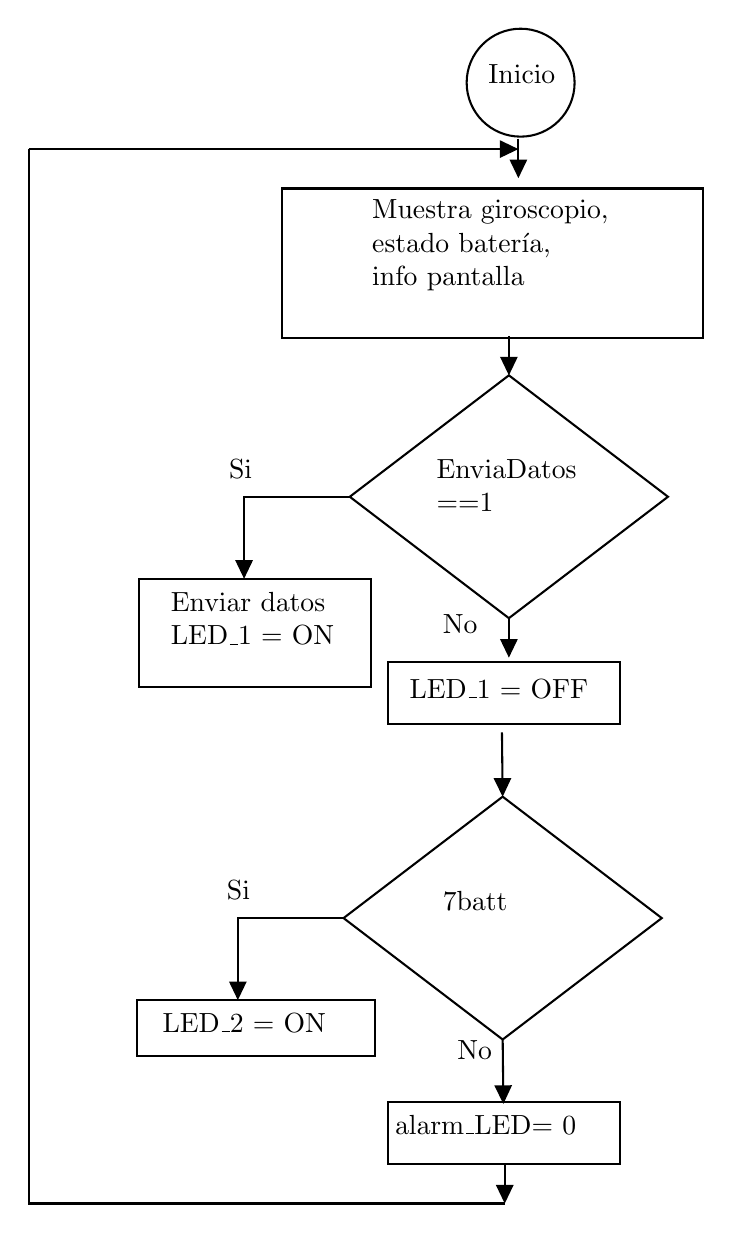
\begin{tikzpicture}[x=0.75pt,y=0.75pt,yscale=-1,xscale=1]
%uncomment if require: \path (0,616); %set diagram left start at 0, and has height of 616

%Flowchart: Connector [id:dp7813495520702245] 
\draw   (315,40) .. controls (315,25.64) and (326.64,14) .. (341,14) .. controls (355.36,14) and (367,25.64) .. (367,40) .. controls (367,54.36) and (355.36,66) .. (341,66) .. controls (326.64,66) and (315,54.36) .. (315,40) -- cycle ;
%Straight Lines [id:da8847526091998554] 
\draw    (339.92,67) -- (339.92,83) ;
\draw [shift={(339.92,86)}, rotate = 270] [fill={rgb, 255:red, 0; green, 0; blue, 0 }  ][line width=0.08]  [draw opacity=0] (8.93,-4.29) -- (0,0) -- (8.93,4.29) -- cycle    ;
%Flowchart: Decision [id:dp21596588394867888] 
\draw   (335.35,181) -- (412,239.5) -- (335.35,298) -- (258.69,239.5) -- cycle ;
%Straight Lines [id:da7204417446380422] 
\draw    (335.35,162) -- (335.35,178) ;
\draw [shift={(335.35,181)}, rotate = 270] [fill={rgb, 255:red, 0; green, 0; blue, 0 }  ][line width=0.08]  [draw opacity=0] (8.93,-4.29) -- (0,0) -- (8.93,4.29) -- cycle    ;
%Straight Lines [id:da49582350632228556] 
\draw    (207.76,260) -- (207.76,276) ;
\draw [shift={(207.76,279)}, rotate = 270] [fill={rgb, 255:red, 0; green, 0; blue, 0 }  ][line width=0.08]  [draw opacity=0] (8.93,-4.29) -- (0,0) -- (8.93,4.29) -- cycle    ;
%Shape: Right Angle [id:dp2914826540765745] 
\draw   (258.69,239.5) -- (207.76,239.5) -- (207.76,260) ;
%Shape: Right Angle [id:dp7943090498770735] 
\draw   (333.35,580) -- (104,580) -- (104,72) ;
%Straight Lines [id:da15691850789793538] 
\draw    (332,353) -- (332.31,381) ;
\draw [shift={(332.35,384)}, rotate = 269.36] [fill={rgb, 255:red, 0; green, 0; blue, 0 }  ][line width=0.08]  [draw opacity=0] (8.93,-4.29) -- (0,0) -- (8.93,4.29) -- cycle    ;
%Flowchart: Process [id:dp025828036440153967] 
\draw   (157,279) -- (269,279) -- (269,331) -- (157,331) -- cycle ;
%Flowchart: Process [id:dp08317044111396199] 
\draw   (226,91) -- (429,91) -- (429,163) -- (226,163) -- cycle ;
%Flowchart: Decision [id:dp9588588712187942] 
\draw   (332.35,384) -- (409,442.5) -- (332.35,501) -- (255.69,442.5) -- cycle ;
%Straight Lines [id:da6075623967992321] 
\draw    (335.35,298) -- (335.35,314) ;
\draw [shift={(335.35,317)}, rotate = 270] [fill={rgb, 255:red, 0; green, 0; blue, 0 }  ][line width=0.08]  [draw opacity=0] (8.93,-4.29) -- (0,0) -- (8.93,4.29) -- cycle    ;
%Straight Lines [id:da7280821078053175] 
\draw    (204.76,463) -- (204.76,479) ;
\draw [shift={(204.76,482)}, rotate = 270] [fill={rgb, 255:red, 0; green, 0; blue, 0 }  ][line width=0.08]  [draw opacity=0] (8.93,-4.29) -- (0,0) -- (8.93,4.29) -- cycle    ;
%Shape: Right Angle [id:dp5301940302382446] 
\draw   (255.69,442.5) -- (204.76,442.5) -- (204.76,463) ;
%Flowchart: Process [id:dp03155186296961898] 
\draw   (156,482) -- (271,482) -- (271,509) -- (156,509) -- cycle ;
%Straight Lines [id:da1967066179049608] 
\draw    (333.35,561) -- (333.35,577) ;
\draw [shift={(333.35,580)}, rotate = 270] [fill={rgb, 255:red, 0; green, 0; blue, 0 }  ][line width=0.08]  [draw opacity=0] (8.93,-4.29) -- (0,0) -- (8.93,4.29) -- cycle    ;
%Flowchart: Process [id:dp5138152311739683] 
\draw   (277,319) -- (389,319) -- (389,349) -- (277,349) -- cycle ;
%Flowchart: Process [id:dp3581810005977748] 
\draw   (277,531) -- (389,531) -- (389,561) -- (277,561) -- cycle ;
%Straight Lines [id:da864404406808954] 
\draw    (332.35,501) -- (332.66,529) ;
\draw [shift={(332.69,532)}, rotate = 269.36] [fill={rgb, 255:red, 0; green, 0; blue, 0 }  ][line width=0.08]  [draw opacity=0] (8.93,-4.29) -- (0,0) -- (8.93,4.29) -- cycle    ;
%Straight Lines [id:da9757080202876469] 
\draw    (104,72) -- (336.92,72) ;
\draw [shift={(339.92,72)}, rotate = 180] [fill={rgb, 255:red, 0; green, 0; blue, 0 }  ][line width=0.08]  [draw opacity=0] (8.93,-4.29) -- (0,0) -- (8.93,4.29) -- cycle    ;

% Text Node
\draw (324,30) node [anchor=north west][inner sep=0.75pt]   [align=left] {Inicio};
% Text Node
\draw (299,220) node [anchor=north west][inner sep=0.75pt]   [align=left] {EnviaDatos\\==1};
% Text Node
\draw (302,295) node [anchor=north west][inner sep=0.75pt]   [align=left] {No};
% Text Node
\draw (199,220) node [anchor=north west][inner sep=0.75pt]   [align=left] {Si};
% Text Node
\draw (171,284) node [anchor=north west][inner sep=0.75pt]   [align=left] {Enviar datos\\LED\_1 = ON};
% Text Node
\draw (268,95) node [anchor=north west][inner sep=0.75pt]   [align=left] {Muestra giroscopio,\\estado batería,\\info pantalla};
% Text Node
\draw (302,428) node [anchor=north west][inner sep=0.75pt]   [align=left] {$\displaystyle 7\geqslant $batt};
% Text Node
\draw (198,423) node [anchor=north west][inner sep=0.75pt]   [align=left] {Si};
% Text Node
\draw (167,487) node [anchor=north west][inner sep=0.75pt]   [align=left] {LED\_2 = ON};
% Text Node
\draw (309,500) node [anchor=north west][inner sep=0.75pt]   [align=left] {No};
% Text Node
\draw (286,326) node [anchor=north west][inner sep=0.75pt]   [align=left] {LED\_1 = OFF};
% Text Node
\draw (279,536) node [anchor=north west][inner sep=0.75pt]   [align=left] {alarm\_LED= 0};


\end{tikzpicture}
\caption{Diagrama de flujo del circuito.}
\label{DF_S}
\end{figure}
Cabe mencionar que, los componentes externos para el sismografo fueron las resistencias y una batería de \SI{9}{\volt}, de donde se hizo un divisor de tensión con una salida de \SI{3.21}{\volt} aproximadamente, lo cual respeta las características mostradas en la figura \ref{fig3}, esto indica que es seguro conectar el cable con esta magnitud a la placa sin problema alguno. En la siguiente sección se mostrará paso a paso su respectivo funcionamiento.
\newpage
